% !TEX spellcheck = en_US
% !TEX TS-program = rakcv
%% single column for submission and review
%\documentclass[journal, onecolumn, 12pt, a4paper, draftcls]{IEEEtran}

%% double column to emulate final version (for submission and review)
\documentclass[10pt, twocolumn, twoside]{IEEEtran}

%% double column for conference
%\documentclass[conference]{IEEEtran}

\IEEEoverridecommandlockouts
\bibliographystyle{IEEEtran}

\usepackage[cmex10]{amsmath} % prevents amsmath from using a Type 3 font for math within footnotes
\interdisplaylinepenalty=2500 % (re)allows page breaks within aligned equations
\usepackage{amssymb}
\usepackage{bm}
\usepackage{mathtools}
\usepackage{cite}
\usepackage{xcolor}
\usepackage{enumerate}
\usepackage{booktabs} % nice table objects
\usepackage{multirow}
\usepackage{lipsum}
\usepackage{graphicx}
\usepackage{breqn}
\usepackage{subcaption}

\usepackage{mathrsfs}
\usepackage{mathtools}
\usepackage{etoolbox}
\usepackage{hyperref}
\usepackage{bibunits}
\usepackage{chngcntr}

\counterwithin*{equation}{section}
\graphicspath{{figs/}{pdf/}{jpg/}{../pdf/}}

%commands
%\renewcommand{\phi}{\varphi}
\newcommand{\untsph}{\mathbb{S}^{2}} % unit sphere
\newcommand{\unit}[1]{\widehat{\bm{#1}}}
\DeclarePairedDelimiterX\abs[1]{\lvert}{\rvert}{#1}
\DeclarePairedDelimiterX\parn[1]{(}{)}{#1}
\DeclarePairedDelimiterX\set[1]{\lbrace}{\rbrace}{#1}
\DeclarePairedDelimiterX\innerp[2]{\langle}{\rangle}{#1,#2}
\DeclarePairedDelimiterX\norm[1]{\lVert}{\rVert}{#1}
\DeclarePairedDelimiterX\brac[1]{[}{]}{#1}
\DeclarePairedDelimiterX\coeff[1]{(}{)}{#1}
\DeclareMathOperator{\expectop}{\mathbb{E}} % \expect[\Big]{ f }
\newcommand{\expect}[2][]{\expectop\set[#1]{#2}}

\newcommand{\figref}[1]{Fig.\,\ref{#1}}
\newcommand{\tabref}[1]{Table~\ref{#1}}
\newcommand{\reals}{\mathbb{R}} % real numbers
\newcommand{\cmplx}{\mathbb{C}} % complex numbers
\newcommand{\dfn}{\triangleq}
\newcommand{\conj}[1]{\overline{#1}} % conjugate
\newcommand{\tendsto}{\rightarrow}

\newtheorem{theorem}{Theorem}%[section]
\renewcommand{\IEEEQED}{\IEEEQEDopen}

\defaultbibliographystyle{IEEEtran}
\defaultbibliography{IEEEabrv,book-collection,sphtriang}

\begin{document}

\title{Single-Taper Window Design on the Sphere}

\ifCLASSOPTIONconference
	\author{
		\IEEEauthorblockN{Rodney~A.~Kennedy}
			\thanks{This research was supported under the Australian Research Council's Discovery Projects
				funding scheme (Project No.~DP150101011).}
		\IEEEauthorblockA{Research School of Engineering,\\
			College of Engineering and Computer Science,\\
			The Australian National University,\\ Canberra, ACT 2601, Australia\\
			Email: rodney.kennedy@anu.edu.au} \and
		\IEEEauthorblockN{Aiden W.~Kennedy}
		\IEEEauthorblockA{Research School of Engineering,\\
			College of Engineering and Computer Science,\\
			The Australian National University,\\ Canberra, ACT 2601, Australia\\
			Email: collaborator@anu.edu.au}}
\else
	\author{Rodney~A.~Kennedy,~\IEEEmembership{Fellow,~IEEE}, and
		Collaborator,~\IEEEmembership{Senior Member,~IEEE}
		\thanks{Rodney~A.~Kennedy and Collaborator are with the Research School of Engineering,
			College of Engineering and Computer Science,
			The Australian National University (ANU), Canberra, ACT 2601, Australia
			(email: $\{$rodney.kennedy, collaborator$\}$@anu.edu.au).}
		\thanks{This work was supported under the Australian Research Council's Discovery Projects
			funding scheme (Project No.~DP1094350).}}
\fi


\maketitle

\newcommand{\R}{\mathscr{R}}
\newcommand{\taper}{w}%{w_{\R}^{\vphantom{g}}}

%\newcommand{\chfn}[2][]{\ifblank{#1}{\chi_{#2}}{\prescript{#1}{}\chi_{#2}}}
\newcommand{\chfn}{\chi_{\R}^{\vphantom{g}}}

\begin{abstract}
These are notes from scattered projects, held in one place a bit like a notebook.
\end{abstract}

\smallskip
\begin{IEEEkeywords}
key, word, keyword list
\end{IEEEkeywords}

\IEEEpeerreviewmaketitle

%\tableofcontents

%\clearpage

\section{Single Taper Design}

\begin{bibunit}


Classes of band-limited tapers for a spherical cap region are developed in \cite{Wieczorek:2005}.

\subsection{Constraints}

Here we seek a single taper $\taper(\unit{x})$ to use as a spatial-multiplicative window for a region $\R\subset\untsph$ on the sphere.  The sought properties are:
\begin{enumerate}
%\item unit energy on the sphere
%\[
%\int_{\untsph} \abs{\taper(\unit{x})}^2\,ds(\unit{x}) = 1
%\]
\item band-limited to degree $L$, that is,
\[
\coeff[\big]{\taper}_{\ell}^{m} = \innerp{\taper}{Y_{\ell}^{m}} = 0,\quad \ell>L,
\]
\item high spatial energy concentration, no less than some threshold $\lambda\in(0,1)$, that is,
\[
\frac{\displaystyle\int_{\R} \abs{\taper(\unit{x})}^2\,ds(\unit{x})}
{\displaystyle\int_{\untsph} \abs{\taper(\unit{x})}^2\,ds(\unit{x})} =
\frac{\norm[\big]{\taper}_{\R}^2}
{\norm[\big]{\taper}^2}
\geq \lambda
\]
and such functions are referred to as $\lambda$-concentrated

\item close to unity in the region of interest, that is, in some sense close to the characteristic function of the region $\R$
\[
\chfn(\unit{x}) =
\begin{cases}
1 & \unit{x}\in\R \\
0 & \text{otherwise}%\unit{x}\in\untsph\setminus\R
\end{cases}
\]
\end{enumerate}

\subsection{Caveats}

\begin{itemize}
\item
The threshold $\lambda\in(0,1)$ should not exceed the maximum theoretical spatial concentration. 

\item
The characteristic function is not band-limited.
\end{itemize}


\subsection{Use of taper}

When performing analysis a signal $f(\unit{x})$ localized to a region $\R$ we propose to use the modified signal
\[
\taper(\unit{x})\,f(\unit{x})
\]
which tends to concentrates the signal simultaneously in the spatial and spectral domains.

\subsection{Band-limited Slepian functions}

The band-limited Slepian functions for region $\R$ are denoted
$\varphi_n(\unit{x})$
with associated real positive eigenvalues $\lambda_n$, $n=1,2,\dotsc$, that is,
\[
\int_{\R} \abs{\varphi_n(\unit{x})}^2\,ds(\unit{x}) = \lambda_n.
\]
The Slepian functions are ordered in $n$ such that
\[
\lambda_n\geq\lambda_{n+1},\quad \forall n.
\]
Further the Slepian functions are orthonormal on $\untsph$ and orthogonal on $\R$.


\newcommand{\band}{s}
\newcommand{\bandt}{\band^{\lambda}}

\subsection{Formulation}

If $\band(\unit{x})$ is an $L$-band-limited function then by the completeness of the band-limited Slepian functions we have
\begin{equation}
\label{eqn:expan}
\band(\unit{x}) =
\sum_{n=1}^\infty \coeff[\big]{\band}_n\,\varphi_n(\unit{x}),
\end{equation}
in the sense of convergence in the mean, where
\begin{equation}
\label{eqn:coeff}
\coeff[\big]{\band}_n =
\innerp{\band}{\varphi_n} =
\int_{\untsph} \band(\unit{x})\,\conj{\varphi_n(\unit{x})}\,ds(\unit{x})
\end{equation}

Define $N(\lambda)$ such that
\begin{equation}
\label{eqn:lambda}
\lambda_{n}\geq \lambda \iff n\leq N(\lambda).
\end{equation}
Then the truncation
\begin{equation}
\label{eqn:expan2}
\bandt(\unit{x}) =
\sum_{n=1}^{N(\lambda)} \coeff[\big]{\bandt}_n\,\varphi_n(\unit{x})
\end{equation}
is $\lambda$-concentrated because we only use the $\lambda$-concentrated $L$-band-limited Slepian functions:
\[
\set[\Big]{\varphi_n(\unit{x})\colon
\int_{\R}\abs[\big]{\varphi_n(\unit{x})}^2\,ds(\unit{x}) = \lambda_n \geq \lambda}{\vphantom{\sum}}_{n=1}^{N(\lambda)}.
\]
That is, by the orthogonality of the Slepian functions on $\R$,
\begin{align*}
\norm[\big]{\bandt}_{\R}^2 &= \int_{\R} \abs[\big]{\bandt(\unit{x})}^{2}\,ds(\unit{x}) \\
&= \sum_{n=1}^{N(\lambda)} \abs[\big]{\coeff[\big]{\bandt}_n}^{2}
\int_{\R}\abs[\big]{\varphi_n(\unit{x})}^2\,ds(\unit{x}) \\
&= \sum_{n=1}^{N(\lambda)} \lambda_{n}\,\abs[\big]{\coeff[\big]{\bandt}_n}^{2}
\geq \lambda\sum_{n=1}^{N(\lambda)}\abs[\big]{\coeff[\big]{\bandt}_n}^{2} = \lambda\, \norm[\big]{\bandt}^2.
\end{align*}

\subsection{Window Design}

Functions satisfying expansion \eqref{eqn:expan2} form a finite $N(\lambda)$-dimensional space of $\lambda$-concentrated signals with the $\lambda$-concentrated $L$-band-limite Slepian functions as their basis.

Now the objective is to find a suitable $\band(\unit{x})$ that does not ``down-weight and ultimately discard'' the signal in the portions of the region $\R$ \cite{Wieczorek:2005}.  A function that equally weights all parts of the region is $\chi_{\R}^{\vphantom{g}}(\unit{x})$, the characteristic function of the region $\R$.  To obtain the optimal minimum mean square error between the inadmissible $\chi_{\R}^{\vphantom{g}}(\unit{x})$ and the finite $N(\lambda)$-dimensional subspace is through an orthogonal projection,
\begin{equation}
\taper(\unit{x}) = \sum_{n=1}^{N(\lambda)} \coeff[\big]{\taper}_n\,\varphi_n(\unit{x})
\end{equation}
where
\begin{align}
\coeff[\big]{\taper}_n = \innerp{\chi_{\R}^{\vphantom{g}}}{\varphi_n}
&= \int_{\untsph} \chi_{\R}^{\vphantom{g}}(\unit{x})\, \conj{\varphi_n(\unit{x})}\,ds(\unit{x}) \nonumber \\
&= \int_{\R} \conj{\varphi_n(\unit{x})}\,ds(\unit{x})
\end{align}

%
%We have by the completeness of the Slepian functions the series for the characteristic function of the region $\R$
%\[
%\chi_{\R}^{\vphantom{g}}(\unit{x}) =
%\sum_{n=1}^\infty \coeff[\big]{\chfn}_n\,\varphi_n(\unit{x})
%\]
%where
%\begin{equation}
%\label{eqn:coeff}
%\coeff[\big]{\chfn}_n =
%\innerp{\chfn}{\varphi_n} =
%\int_{\R} \conj{\varphi_n(\unit{x})}\,ds(\unit{x})
%\end{equation}
%
%Then we form the truncated series
%\begin{equation}
%\label{eqn:wind}
%\chi_{\R}^{N(\lambda)}(\unit{x}) = \sum_{n=1}^{N(\lambda)} \coeff[\big]{\chfn}_n\,\varphi_n(\unit{x})
%\end{equation}
%where $N(\lambda)$ is such that
%\begin{equation}
%\label{eqn:lambda}
%\lambda_{n}\geq \lambda \iff n\leq N(\lambda).
%\end{equation}
%
%The spatial concentration of $\chi_{\R}^{N(\lambda)}(\unit{x})$ can be bounded as follows.  Firstly we evaluate the energy in the region
%\begin{align*}
%\int_{\R} \abs[\big]{\chi_{\R}^{N(\lambda)}(\unit{x})}^{2}\,ds(\unit{x})
%&= \sum_{n=1}^{N(\lambda)} \abs[\big]{\coeff[\big]{\chfn}_n}^{2} \int_{\R}
%\,\abs[\big]{\varphi_n(\unit{x})}^2\,\,ds(\unit{x}) \\
%&= \sum_{n=1}^{N(\lambda)} \lambda_{n}\,\abs[\big]{\coeff[\big]{\chfn}_n}^{2} \\
%&\geq \lambda\sum_{n=1}^{N(\lambda)}\abs[\big]{\coeff[\big]{\chfn}_n}^{2},
%\end{align*}
%where we have applied the uniform bound on $\lambda_n$.
%
%Similarly the energy on the whole sphere is
%\begin{align*}
%\int_{\untsph} \abs[\big]{\chi_{\R}^{N(\lambda)}(\unit{x})}^{2}\,ds(\unit{x})
%%&= \sum_{n=1}^{N(\lambda)} \abs[\big]{\coeff[\big]{\chfn}_n}^{2} \int_{\untsph}
%%\,\abs[\big]{\varphi_n(\unit{x})}^2\,\,ds(\unit{x}) \\
%&=
%\sum_{n=1}^{N(\lambda)} \abs[\big]{\coeff[\big]{\chfn}_n}^{2},
%\end{align*}
%which is the Parseval relation.
%
%Then the spatial energy concentration satisfies
%\[
%\frac{\displaystyle\int_{\R} \abs[\big]{\chi_{\R}^{N(\lambda)}(\unit{x})}^{2}\,ds(\unit{x})}
%{\displaystyle\int_{\untsph} \abs[\big]{\chi_{\R}^{N(\lambda)}(\unit{x})}^{2}\,ds(\unit{x})} \geq
%\lambda
%\]

%\subsection{Window construction}
%
%In summary, from \eqref{eqn:coeff}, \eqref{eqn:wind} and \eqref{eqn:lambda}), we define
%\[
%\taper(\unit{x}) =
%\chi_{\R}^{N(\lambda)}(\unit{x}),
%\]
%which is the truncated, normalized Slepian function expansion of the characteristic function of the region $\R$.  This is a single taper that satisfies the desired properties.

\putbib
\end{bibunit}

\end{document}

\clearpage

\newcommand{\T}{\mathscr{T}\!}
\newcommand{\proj}{\mathscr{B}}

%: 

\section{Integration on Spherical Triangles}
\begin{bibunit}

We consider integration over spherical polygon regions of the unit sphere, $\proj\in\untsph$, whose boundaries are great circles.  Because such regions can be considered as the union of a finite number of spherical triangles, which are in-turn bounded by three great circles, then it is sufficient to consider integration over an arbitrary spherical triangle, $\T\subset\untsph$.  So the fundamental problem we consider is determining
\[
\int_{\T} f(\unit{x})\,ds(\unit{x})
= \int_{\T} f(\theta,\varphi)\,\sin\theta\,d\theta\,d\varphi
\]
for some complex-valued function $f\colon \untsph\supset\T\mapsto\mathbb{C}$.

\subsection{Motivating Examples}

In applications the following problems arise, which highlight that when the integrand involves a spherical harmonic, $Y_{\ell}^{m}(\unit{x})$, or its conjugate, $\conj{Y_{\ell}^{m}(\unit{x})}=(-1)^{m}Y_{\ell}^{-m}(\unit{x})$, then there is particular interest.

\subsubsection{Case 1} The integration over $\T$ of some $f(\unit{x})$ that admits an expansion in spherical harmonics
\begin{equation}
\label{eqn:prob1}
\int_{\T} f(\unit{x})\,ds(\unit{x}), \text{~where~}
f(\unit{x}) = \sum_{\ell,m} (f)_{\ell}^{m} Y_{\ell}^{m}(\unit{x}),
\end{equation}
with Fourier coefficients
\[
(f)_{\ell}^{m}=\innerp[\big]{f}{Y_{\ell}^{m}}
=\int_{\untsph} f(\unit{x})\,\conj{Y_{\ell}^{m}(\unit{x})}\,ds(\unit{x})
\]
obtained through the spherical harmonic transform.  Further, by truncating the Fourier series expansion in degree $\ell$, provides a convenient way to smooth the integrand.

\subsubsection{Case 2} A function may be spatially masked to triangle $\T$ through a projection operator $\proj_{\T}$ and the spherical harmonic transform of the result gives
\begin{align}
\coeff{\proj_{\T}f}_{\ell}^{m}
&=\int_{\untsph} \parn[\big]{\proj_{\T}f}(\unit{x})\,
\conj{Y_{\ell}^{m}(\unit{x})}\,ds(\unit{x})\nonumber\\
&=\int_{\T} f(\unit{x})\,\conj{Y_{\ell}^{m}(\unit{x})}\,ds(\unit{x})\label{eqn:prob2}
\end{align}
In this case the projection operator $\proj_{\T}$ may model a process where there is incomplete measurements on the sphere.


\subsubsection{Case 3} In the case where the region of interest is $\T$ then the following Gramian is fundamental when determining the Slepian functions for $\T$
\begin{equation}
\label{eqn:prob3}
\int_{\T} Y_{p}^{q}(\unit{x})\,\conj{Y_{\ell}^{m}(\unit{x})}\,ds(\unit{x})
\end{equation}
and it also arises in combining the spherical harmonic expansion in \eqref{eqn:prob1} with \eqref{eqn:prob2}.

In summary, the fundamental entity to be evaluated is
\begin{equation}
\label{eqn:prob4}
\int_{\T} Y_{\ell}^{m}(\unit{x})\,ds(\unit{x}).
\end{equation}

\begin{figure}[tb]
\centering
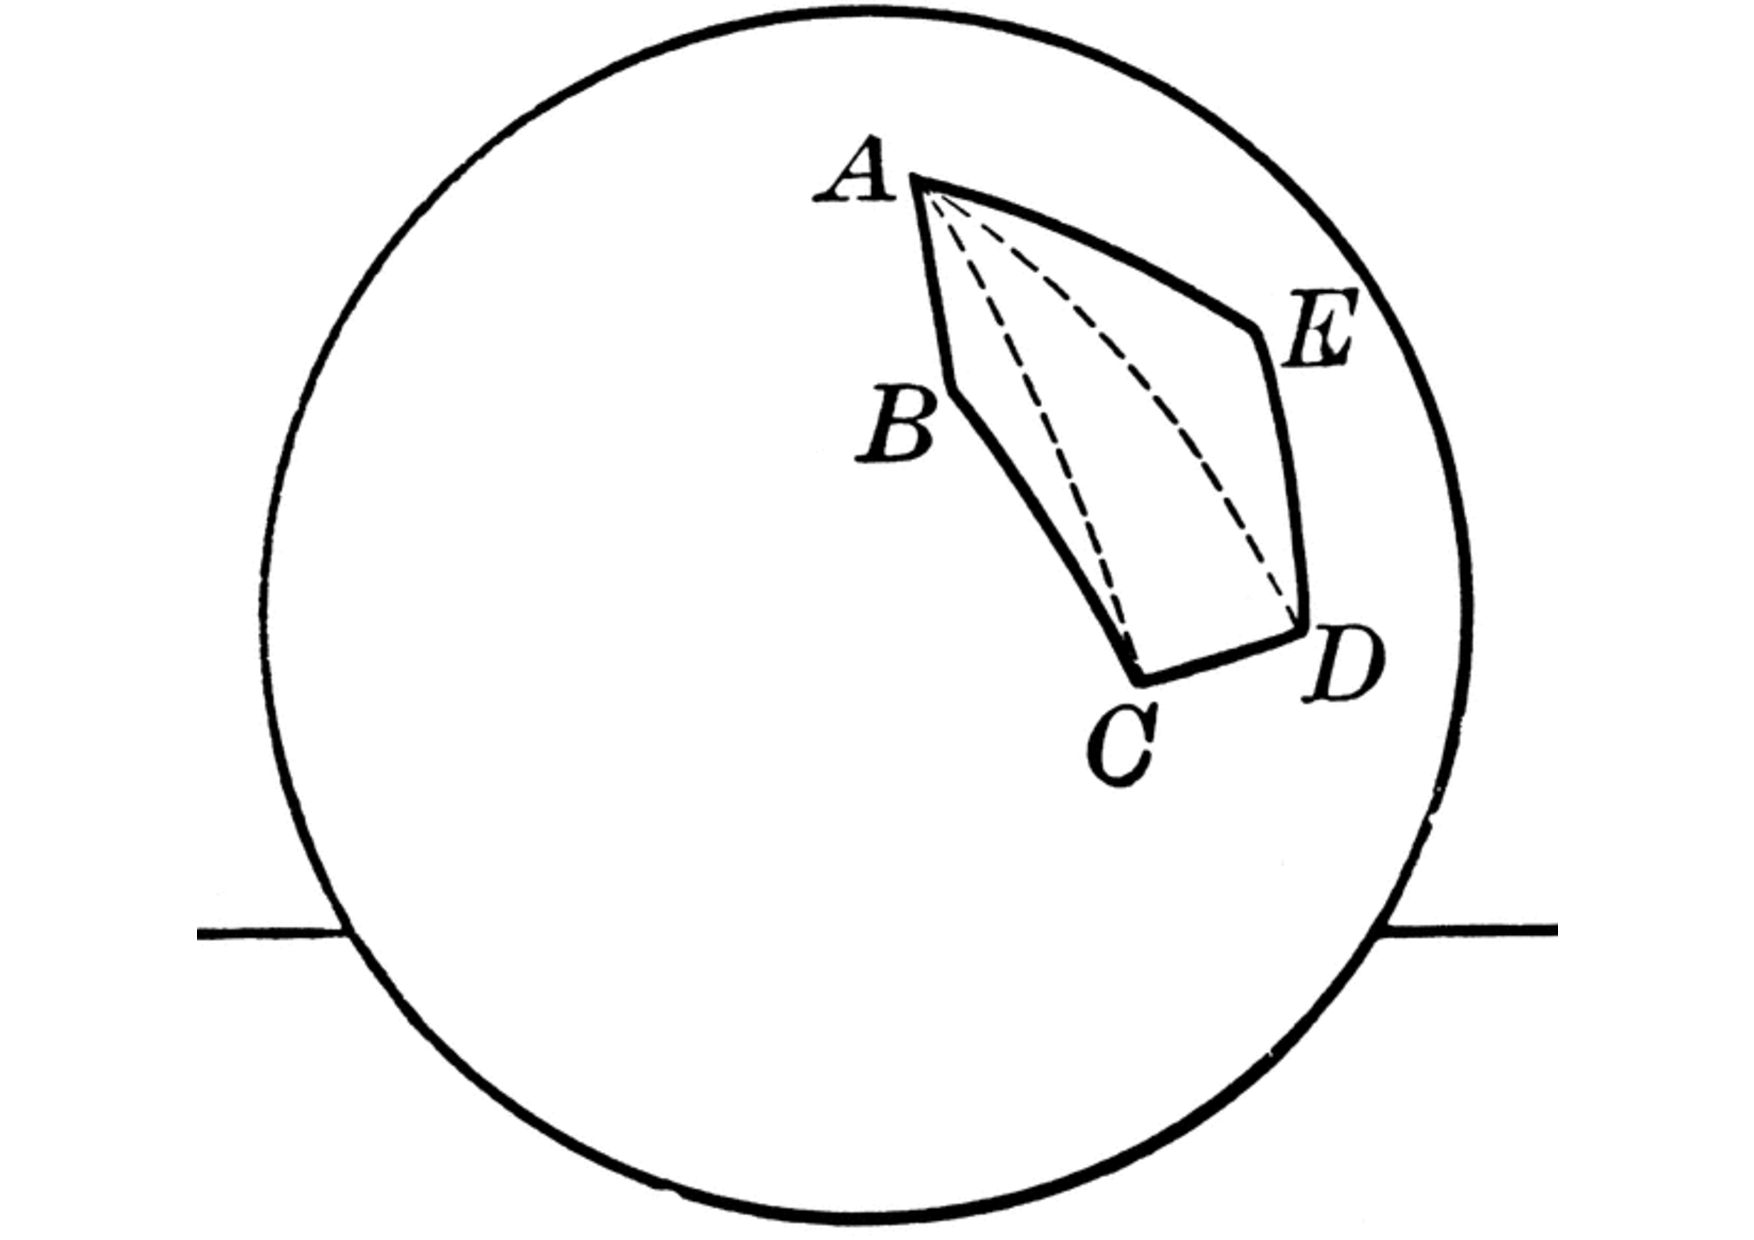
\includegraphics[width=0.8\columnwidth]{pdfs/spherepoly.pdf}
\end{figure}

\subsection{Right equatorial triangles}

In the spherical coordinate system, an SO(3) rotation can map a spherical triangle $\T$ to bring one of its edges to lie along the equator, where $\theta=\pi/2$, with one vertex $A$ at $\phi=0$ and the other vertex $B$ at $\phi=\phi_B$.  The third vertex $C$ can be taken anywhere in the northern hemisphere ($0<\theta_C<\pi/2$).  We describe such triangles as ``equatorial triangles''.  A special case is the ``right equatorial triangles'' when the vertex C is at $\phi_C=0$ such that it forms a right triangle with vertices $A$ and $B$.  The more general (non-right) spherical triangle $\T$ can be seen to be a sum or difference of two right triangles.  Hence it is sufficient to consider integration of a right equatorial triangle whose vertices are given by $A\colon(1,0,0)$, $B\colon(1,0,\phi_B)$ and $C\colon(1,\theta_C,0)$ where the parameters are spherical polars $(\rho,\theta,\phi)$.  That is, integration over a spherical polygon can be reduced to the problem of integration over right equatorial triangles.

In essence we are saying 
\[
	\T = \mathcal{R}(\alpha,\beta,\gamma)(\T_0\pm\T_1)
\]
where $\T_0$ and $\T_1$ are right equatorial triangles.

\subsection{Triangulation}




\subsection{Comparison with other approaches}

Numerical approach is given in \cite{Sanchez:2004}

\putbib
\end{bibunit}

\clearpage

%: 
\section{Diffusion Modeling and Visualization}

\newcommand{\newurl}[1]{{\small\color{blue!80!black}\ttfamily\bfseries\url{#1}}}

\subsection{Basic model}

To model molecular diffusion in a non-homogeneous and non-isotropic medium we quantize an irregular portion of 3D space into cubes.  Molecules move across each of 6 faces of a cube according to the relative concentration across each of the faces and also subject to a spatially dependent diffusion coefficient (as a consequence of the non-homogeneous and non-isotropic medium).  Molecules move through space and therefore between cubes. At least one cube is a source and other cubes (such as boundary cubes) can act as sinks.

Each cube has a state that counts the number of molecules inside the cube (length of queue).  This state is probabilistically updated each iteration based on the current state and the states of the 6 nearest neighbor cubes.  There are a number of ways to model how this update takes place and generally the update is not computationally intensive.

\subsection{Visualization}

Mayavi (\newurl{http://mayavi.sourceforge.net}) is a python wrap to VTK (\newurl{http://www.vtk.org}), an open-source, freely available software system for 3D computer graphics, image processing and visualization.  It readily supports 3D scene rendering.  To each scene voxel we can associate a cube state.  We can visualize the time evolution of the state through time changing iso-surfaces of the molecular concentration.  There are a number of ways of representing this spatial information, as well as iso-surfaces, we could use volume rendering or point clouds, see \newurl{http://docs.enthought.com/mayavi/mayavi/mlab_case_studies.html}.  Further we can encode information into the color of voxels and their opacity.  High molecular concentrations should have higher opacity and deeper colors.  Multiple

Julia (\newurl{http://julialang.org}) also can access through Mayavi.  The visualization engine is VTK and languages such a Python and Julia only need serve as a higher level interface and don't impact the 3D rendering speed, which is ultimately up to the GPU and graphic card.  Julia is designed for high speed technical computing and use in the computational aspects.

\subsection{Animation}

\newurl{http://docs.enthought.com/mayavi/mayavi/mlab_animating.html\#mlab-animating-data}




%\bibliography{IEEEabrv,book-collection}

\end{document}



\newpage
\section{Conclusions}

\lipsum[28]

\bibliography{IEEEabrv,wSlepian}

\appendices

\section{Obscure Thing}

\lipsum[38]

\section{Unclear Thing}

\lipsum[41]

\end{document}

